\section{Background and Motivation}\label{sec:motivation}

In this section, we first introduce how ECMA-262~\cite{es13} describes
JavaScript syntax and semantics with simple examples.
%
Then, we explain how prior work synthesizes JavaScript conformance tests using
coverage-guided fuzzing~\cite{afl} with the control-flow graph (CFG) in the
language specification.
%
Finally, we explain why node/branch coverages cannot fully discriminate
different semnatics in different language features or even in the same features.

\subsection{JavaScript Language Specification (ECMA-262)}

\begin{figure}
  \centering
  \begin{subfigure}{\textwidth}
    \[
      \begin{array}{l}
        \esntp{AdditiveExpression}{Yield, Await} \est{:}\\

        \qquad \esntp{MultiplicativeExpression}{?Yield, ?Await}\\

        \qquad \esntp{AdditiveExpression}{?Yield, ?Await} \; \est{+} \;
        \esntp{MultiplicativeExpression}{?Yield, ?Await}\\

        \qquad \esntp{AdditiveExpression}{?Yield, ?Await} \; \est{-} \;
        \esntp{MultiplicativeExpression}{?Yield, ?Await}\\
      \end{array}
    \]
    \subcaption{The syntax defined with a variant of EBNF.}
  \end{subfigure}
  \par\bigskip
  \begin{subfigure}{\textwidth}
    \textbf{13.8.1.1 Runtime Semantics: Evaluation}
    \\%
    \esnt{AdditiveExpression} \est{:} \esnt{AdditiveExpression} \est{+}
    \esnt{MultiplicativeExpression}
    \vspace*{.5em}\\%
    1. Return ?${}^{2}$
    \esalg{EvaluateStringOrNumericBinaryExpression}${}^{1}$(\esnt{AdditiveExpression},
    \escode{+}, \esnt{MultiplicativeExpression}).${}^{3}$
    \\%

    \textbf{13.8.2.1 Runtime Semantics: Evaluation}
    \vspace*{.5em}\\%
    \esnt{AdditiveExpression} \est{:} \esnt{AdditiveExpression} \est{-}
    \esnt{MultiplicativeExpression}
    \vspace*{.5em}\\%
    1. Return ?${}^{5}$
    \esalg{EvaluateStringOrNumericBinaryExpression}${}^{4}$(\esnt{AdditiveExpression},
    \escode{-}, \esnt{MultiplicativeExpression})${}^{6}$.
    \\%

    \textbf{13.15.4 EvaluateStringOrNumericBinaryExpression (
      \esvar{leftOperand},
      \esvar{opText},
      \esvar{rightOperand}
    )}
    \vspace*{.5em}\\%
    % 1. Let \esvar{lref} be the result of evaluating \esvar{leftOperand}.
    % \\%
    % 2. Let \esvar{lval} be ? \esalg{GetValue}(\esvar{lref}).
    % \\%
    % 3. Let \esvar{rref} be the result of evaluating \esvar{rightOperand}.
    % \\%
    % 4. Let \esvar{rval} be ? \esalg{GetValue}(\esvar{rref}).
    ...${}^{7}$
    \\%
    5. Return ?${}^{9}$ \esalg{ApplyStringOrNumericBinaryOperator}${}^{8}$(\esvar{lval},
    \esvar{opText}, \esvar{rval}).${}^{10}$
    \\%

    \textbf{13.15.3 ApplyStringOrNumericBinaryOperator (
      \esvar{lval},
      \esvar{opText},
      \esvar{rval}
    )}
    \vspace*{.5em}\\%
    % 1. If \esvar{opText} is \escode{+}, then ...
    % \\%
    % 2. NOTE: At this point, it must be a numeric operation.
    ...${}^{11}$
    \\%
    3. Let \esvar{lnum} be ?${}^{13}$ \esalg{ToNumeric}${}^{12}$(\esvar{lval}).
    \\%
    4. Let \esvar{rnum} be ?${}^{15}$ \esalg{ToNumeric}${}^{14}$(\esvar{rval}).
    \\%
    5. If \esalg{Type}(\esvar{lnum}) is different from \esalg{Type}(\esvar{rnum})${}^{16}$,
    \cfbox{red}{throw a \esval{TypeError} exception.}${}^{\inred{17}}$
    \\%
    ...${}^{18}$
    \\%

    \textbf{7.1.3 ToNumeric ( \esvar{value} )}
    \vspace*{.5em}\\%
    % 1. ${}^{19}$Let \esvar{primValue} be ? \esalg{ToPrimitive}(\esvar{value},
    % \esconst{number}).
    ...${}^{19}$
    \\%
    2. If \esalg{Type}(\esvar{primValue}) is BigInt${}^{20}$, \cfbox{red}{return
    \esvar{primValue}.}${}^\inred{21}$
    \\%
    ...${}^{20}$
    \\%

    % \textbf{22.1.3.14 String.prototype.normalize ( [ \esvar{form} ] )}
    % \vspace*{.5em}\\%
    % 1. Let \esvar{O} be ? \esalg{RequireObjectCoercible}(\esval{this} value).
    % \\%
    % 2. Let \esvar{S} be ? \esalg{ToString}(\esvar{O}).
    % \\%
    % 3. If \esvar{form} is \esval{undefined}, let \esvar{f}\;  be \esval{"NFC"}.
    % \\%
    % 4. Else, let \esvar{f}\; be ? \esalg{ToString}(\esvar{form}).
    % \\%
    % ...
    % \\%
    % 
    % \textbf{ToString ( \esvar{argument} )}
    % \vspace*{.5em}\\%
    % % 1. If \esalg{Type}(\esvar{argument}) is Undefined, return \esval{"undefined"}.
    % % \\%
    % % 2. Else if \esalg{Type}(\esvar{argument}) is Null, return \esval{"undefined"}.
    % % \\%
    % % 3. Else if \esalg{Type}(\esvar{argument}) is Boolean,
    % % \\%
    % % \indent a. If \esvar{argument} is \esval{true}, return \esval{"true"}.
    % % \\%
    % % \indent b. If \esvar{argument} is \esval{false}, return \esval{"false"}.
    % % \\%
    % % 4. Else if \esalg{Type}(\esvar{argument}) is Number, return
    % % \esalg{Number::toString}(\esvar{argument}).
    % ...
    % \\%
    % 5. Else if \esalg{Type}(\esvar{argument}) is String, return \esvar{argument}.
    % \\%
    % ...
    % % 6. Else if \esalg{Type}(\esvar{argument}) is Symbol, throw a \esval{TypeError}
    % % exception.
    % % \\%
    % % 7. Else if \esalg{Type}(\esvar{argument}) is BigInt, return !
    % % \esalg{BigInt::toString}(\esvar{argument}).
    % % \\%
    % % 8. Else if \esalg{Type}(\esvar{argument}) is Object,
    % % \\%
    % % \indent a. Let \esvar{primValue} be ? \esalg{ToPrimitive}(\esvar{argument},
    % % \esval{string}).
    % % \\%
    % % \indent b. Return ? \esalg{ToString}(\esvar{primValue}).
    % \\%
    \subcaption{The semantics defined with abstract algorithms.}
  \end{subfigure}
  \caption{
    The (a) syntax and (b) semantics of \esnt{AdditiveExpression} for addition
    (\scode{+}) and subtraction (\scode{-}) operators described in the latest
    JavaScript language specification (ES13, 2022).
  }
  \label{fig:spec-additive}
\end{figure}

\begin{figure}
  \centering
  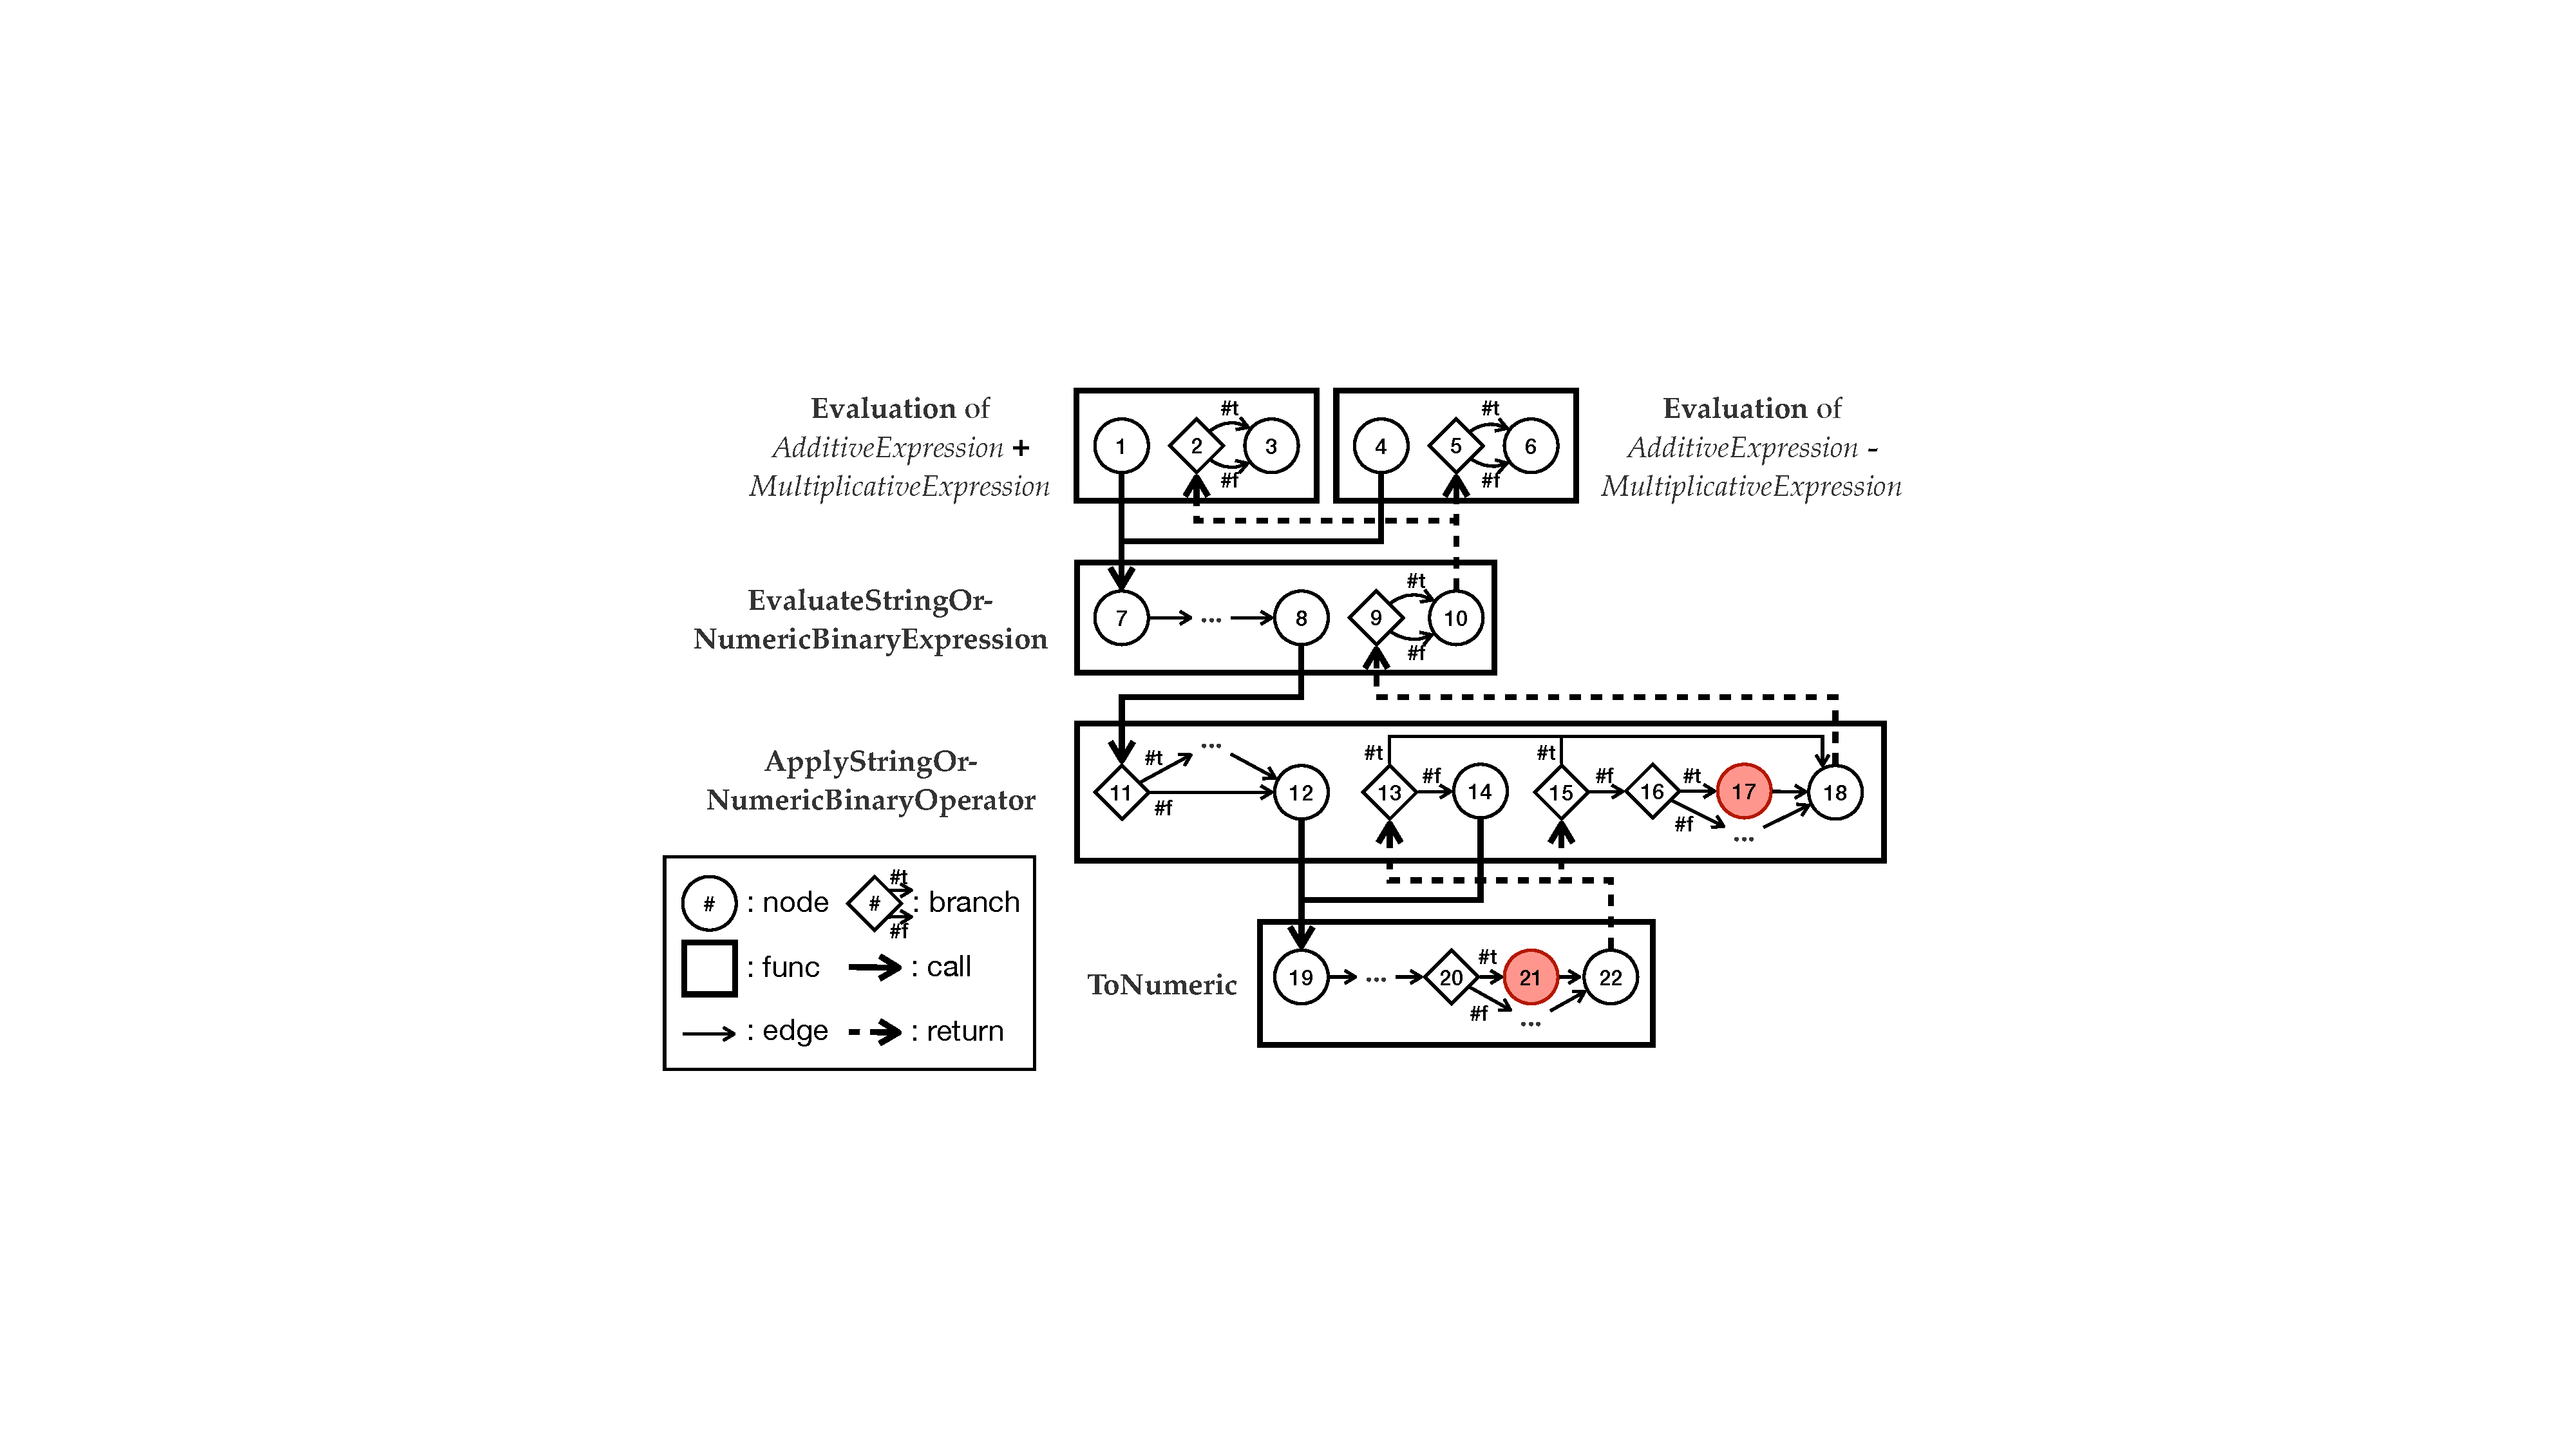
\includegraphics[width=\textwidth]{img/spec-cfg}
  \caption{
    The control-flow graph (CFG) for two different \textbf{Evaluation}
    algorithms of \esnt{AdditiveExpression} for addition (\scode{+}) and
    subtraction (\scode{-}) operators in ES13.
  }
  \label{fig:spec-cfg}
\end{figure}

\todo
